% !TEX root = main.tex

\newpage
\appendix

%%%% Title Page

\pagecolor{mygray}

\begin{titlepage}
   \begin{center}
       \vspace*{6cm}
       {\fontsize{40pt}{46pt}\selectfont \textbf{Appendices}}\\          
   \end{center}
\end{titlepage}

\pagecolor{white}


\begin{appendices}

%\addcontentsline{toc}{section}{Appendices}
\addchap{Appendices}


%%%%%%%%%%%%%%%%%%%%%%% APPENDICES CHAPTER 1 %%%%%%%%%%%%%%%%%%%%%%%


\renewcommand{\thesection}{1.\arabic{section}}



%%%%%%%%%%%%%% NEWSPAPER ARTICLES COLOUR CHANGES %%%%%%%%%%%%%%

\section[\hspace{0.3cm}Newspaper articles on colour changes in works of art]{ Appendix: Newspaper articles on colour changes in works of art}
\label{app:ch1_articles_lid}

\begin{itemize}
    \item February 7, 2020 - New York Times
    
    \textit{‘The Scream’ Is Fading. New Research Reveals Why}. By Sophie Haigney
    
    The art world is increasingly turning to scientific analysis of pigments to find out how time has changed some famous paintings.

    \href{https://www.nytimes.com/2020/02/07/arts/design/the-scream-edvard-munch-science.html}{Link New York Times article}\\
       

    \item June 1, 2018 - New York Times
    
    \textit{Van Gogh’s Yellow ‘Sunflowers’ Could Start to Turn Olive Green}. By Nina Siegal
    
    A pigment the painter used in the work is very sensitive to light and has a tendency to turn to a green hue over time, the authors of a technical study say.
        
    \href{https://www.nytimes.com/2018/06/01/arts/design/van-gogh-yellow-sunflowers.html}{Link New York Times article}\\


    \item May 21, 2015 - New York Times   
    
    \textit{Review: ‘Van Gogh: Irises and Roses,’ Sheds Light on a Disappearing Red Hue}. By Roberta Smith
    
    Technology helps curators and conservators understand a synthetic red pigment and how it changed in paintings we thought we knew, at the Metropolitan Museum of Art.    
  
    \href{https://www.nytimes.com/2015/05/22/arts/design/review-van-gogh-irises-and-roses-sheds-light-on-a-disappearing-red-hue.html}{Link New York Times article}\\

    
    \item May 2, 2013 - The Guardian

    \textit{Van Gogh's true colours were originally even brighter}. By Jonathan Jones

    Research undertaken by the Van Gogh Museum reveals the master's favourite paints have faded badly since the 1880s

    \href{https://www.theguardian.com/artanddesign/jonathanjonesblog/2013/may/02/van-gogh-original-colours-brighter}{Link The Guardian article}

\end{itemize}


%%%%%%%%%%%%%% TIMELINE AND LIST VGM RESEARCH PROJECTS %%%%%%%%%%%%%%

\begin{landscape}
\newpage
\section[\hspace{0.3cm}Timeline and list of past research projects at the Van Gogh Museum]{ Appendix: Timeline and list of past research projects at the Van Gogh Museum}
\label{app:ch1_timeline_VGM-projects}

\vspace{5cm}

\begin{figure}[!h]
\centering
\includegraphics[scale=0.25]{Appendices/Figures/VGM_chronological_chart.png}
\caption*{Timeline of research projects on colour changes.}
\end{figure}  

\end{landscape}


\newpage
%\section[\hspace{0.3cm}List of past research projects at the Van Gogh Museum]{ Appendix: List of past research projects at the Van Gogh Museum}
%\label{app:ch1_list_VGM-projects}




\begin{table}[!h]
\centering
\caption*{Publications related to each project mentioned in Appendix \ref{app:ch1_timeline_VGM-projects}.}
\begin{tabular}{C{2cm}C{4.5cm}C{7cm}}
\toprule[0.4mm]
\textbf{Project} & \textbf{Research type} & \textbf{Publications} \\\midrule
\acrshort{CL} condition surveys & materials characterisation & Internal report submitted by V.R. Mehra to the Van Gogh Museum in 1986 (see \citep[p.35, note  53]{hendriks_vincent_2011})\\\hline
\acrshort{CL} analyses & materials characterisation &  (Cahier Vincent 3) \citep{hofenk_de_graaff_scientific_1991} \\\hline
Shell Research NL\textsuperscript{a} & historical research, materials characterisation & \citep{hendriks_vincent_2011})\\\hline
\multirow{3}{2cm}{\centering Red lakes project} & materials characterisation & \citep{bommel_investigation_2005}  \\
 & art technology & \citep{kirby_reconstruction_2005} \\
 & degradation understanding & \citep{burnstock_comparison_2005,van_den_berg_fading_2006}  \\\hline
The Bedrooms project &  historical research, materials characterisation, prediction & \citep{hendriks_comparative_2011,fiedler_materials_2016, berns_digital_2019} \\\hline
The Sunflowers project & materials characterisation, degradation understanding, art technology, historical research & \citep{monico_degradation_2011, monico_degradation_2011-1, monico_degradation_2012, monico_degradation_2013, monico_degradation_2011-1, monico_evidence_2015, vanmeert_chemical_2018,hendriks_van_2019}\\\hline
\gls{REVIGO} project & art technology, materials characterisation, prediction & \citep{kirchner_digitally_2017, kirchner_digitally_2017-1, kirchner_digitally_2018, geldof_reconstructing_2018} \\\hline
VGM-ASML Partnership in Science & art technology, materials characterisation, degradation understanding & Publications to come \\
\bottomrule[0.4mm]
\end{tabular}
\label{tab:VGM_projects_list}
\footnotesize{\\ \textsuperscript{a} The Van Gogh Museum started to collaborate with Shell Research NL from 2000 to 2018. This collaboration provided suppport for the Red Lakes project and for the series of catalogues of the Van Gogh works (drawings and paintings) in the collection.}
\end{table}




%%%%%%%%%%%%%% RED LAKES PROJECT %%%%%%%%%%%%%%

\newpage
\section[\hspace{0.3cm}Summary of the Red Lakes project]{ Appendix: Summary of the Red Lakes project}
\label{app:ch1_Red-lake_project}


Between 2000 and 2005, the "Red Lakes project" took place under the leadership of the Van Gogh Museum and the Instituut Collectie Nederland and with the collaboration of the Shell Research and Technology Centre, Amsterdam, the Courtauld Institute of Art and the National Gallery, London. The project started with detailed examination of 93 paintings of the Antwerp and Paris periods of Van Gogh (November 1885 - February 1888) in the context of the new collection catalogue volume 2 \citep{hendriks_vincent_2011}. The aim of these observations, performed by Ella Hendriks and Natasha Duff, was to categorize the different types of red lakes used by Van Gogh in a timeline and report on their methods of application and condition states. The results of the visual inspection were then related to chemical analyses of microscopic paint samples performed by Maarten van Bommel and Muriel Geldof \citep{bommel_investigation_2005}. This approach has been continued for Cat.3 (1888-1890 paintings) with the added possibility of macro-XRF scanning of all paintings. The publication of this last catalogue in the series is expected in 2024. The steps of examination and analysis revealed the predominant use of five red lakes - cochineal on tin substrate, cochineal on calcium and aluminum substrate, madder, eosin (both on aluminum substrate), and brazilwood. The chemical composition, colour and morphology of pigment particles observed in paint cross-sections were cross-related to historical research on red lake fabrication recipes \citep{kirby_reconstruction_2005}. This third stage of the project was led by Klaas Jan van den Berg, and involved three parts: i) creation of pigments, including all the lakes mentioned above using 19\textsuperscript{th} century French and German recipes, under the supervision of Jo Kirby \citeyear{kirby_reconstruction_2005} ; ii). Creation of model paint-outs under the supervision of Leslie Carlyle \citep{carlyle_reconstructions_2020}; iii) studying the fading characteristics of the paints under the supervision of Klaas Jan van den Berg \citep{burnstock_comparison_2005,van_den_berg_fading_2006}. The results showed that brazilwood and eosin samples were the most light sensitive, in the most extreme case showing complete loss of colour after 500 hours of experimental exposure with an illuminance of 10 000 lux - equivalent to less than 10 years of ageing under museum conditions (with an illuminance value of 150 lux and an exposure duration of 3600 hours per year, equivalent to a display of 10 hours per day for 360 days). Finally, to return full circle, a selection of Van Gogh’s paintings were re-examined in the light of experimental results to see if the artificially aged samples showed phenomena equivalent to what is seen on the naturally aged paintings. For instance, both the samples and paintings showed increased fading when the paint was applied on a light reflective substrate, or the red pigment was mixed with white pigment that increased the scattering of light within the paint film \citep[p.463-465]{burnstock_comparison_2005}. As a whole, the project set an example of working methodology for future research projects examining similar issues. In retrospect, it can be said that an important outcome of this study was to determine criteria that can be used for visual identification of the different types of red lake used in Van Gogh’s paintings without having to take samples (based on UV fluorescence, colour, transparency, paint rheology, characteristic degradation phenomena, etc.). Also, spurred by this study, new non-invasive analytical techniques have since been developed for the identification and mapping of red lakes used in Van Gogh’s paintings. 

\end{appendices}




%%%%%%%%%%%%%%%%%%%%%%% APPENDICES CHAPTER 3 %%%%%%%%%%%%%%%%%%%%%%%

\begin{appendices}
  
\renewcommand{\thesection}{3.\arabic{section}}


%%%%%%%%%%%%%% NAMING CONVENTIONS %%%%%%%%%%%%%%

\newpage
\section[\hspace{0.3cm}Naming conventions]{ Appendix: Naming convention for files}
\label{app:ch3_naming_conventions}

\underline{Micro-fading analyses}


\textit{date}\_\textit{Id n$^\circ$}\_\textit{paint code}\_\textit{pigments}\_\textit{lamp}\_\textit{measurement option}\_\textit{filter}\_$d_{ill}$\_\textit{optical fibre}\_SP.csv

\textit{date}\_\textit{Id n$^\circ$}\_\textit{paint code}\_\textit{pigments}\_\textit{lamp}\_\textit{measurement option}\_\textit{filter}\_$d_{ill}$\_\textit{optical fibre}\_dE.csv

\textit{date}\_\textit{Id n$^\circ$}\_\textit{paint code}\_\textit{pigments}\_\textit{lamp}\_\textit{measurement option}\_\textit{filter}\_$d_{ill}$\_\textit{optical fibre}\_INFO.txt\\

\underline{Reflectance measurements}

\textit{date}\_\textit{Id n$^\circ$}\_\textit{sample n$^\circ$}\_\textit{paint code}\_\textit{pigments}\_\textit{experiment}\_\textit{background}\_\textit{device}.txt\\

\underline{Power measurements}

\textit{date}\_\textit{Id n$^\circ$}\_\textit{lamp}\_\textit{measurement option}\_\textit{filter}\_$d_{ill}$\_\textit{optical fibre}.txt\\


\underline{Absolute irradiance measurements}

\textit{date}\_\textit{Id n$^\circ$}\_\textit{lamp}\_\textit{measurement option}\_\textit{filter}\_$d_{ill}$\_\textit{optical fibre}\_\textit{device}.txt\\



%%%%%%%%%%%%%% 3D PRINTS DESCRIPTION %%%%%%%%%%%%%%

\newpage
\section[\hspace{0.3cm}3D prints description]{ Appendix: 3D prints description}
\label{app:ch3_3D-prints}

In total, nine 3D prints have been added to the stereo-MFT in order to connect different parts (Table below). A stl file is available for each 3D print and can be opened with the open source software called \textit{FreeCad}. The FCStd files are available on a Zenodo repository via the the following url : \url{https://doi.org/10.5281/zenodo.7835190} \\

\begin{table}[!h]
\centering
\caption*{Description of the 3D prints used in the stereo-MFT.}
\begin{tabular}{C{1.5cm}C{3cm}C{2cm}C{7cm}}
\toprule[0.4mm]
\textbf{3D print N$^\circ$} & \textbf{Position} & \textbf{Photos} & \textbf{Function} \\\midrule
1 & \multirow{2}{3cm}{\centering Left binocular} & \multirow{2}{*}{\centering Figures (a) \& (e)} & Connection with the optical fibre of the fading light source  \\
2 & & & Possibility to insert filters \\\hline
3 & \multirow{2}{3cm}{\centering Right binocular} & \multirow{2}{*}{\centering Figures (a) \& (e)} & Connection with the optical fibre of the spectrometer \\
4 & & & Possibility to insert filters \\\hline
5 & Phototube S & Figure (c) & Connection with camera \\\hline
6 & \multirow{4}{3cm}{\centering Common main objective} & \multirow{4}{2cm}{\centering Figures (b) \& (d)} & \multirow{4}{7cm}{\centering Connection with the focusing head which is attached to the colour measurement light source}\\
7 & & & \\
8 & & & \\
9 & & & \\
\bottomrule[0.4mm]
\end{tabular}
\label{tab:sMFT_3D-prints}
\end{table}


\vspace{2cm}



\begin{figure}[!h]
\centering
\includegraphics[width=0.9\textwidth]{Appendices/Figures/Fig01_3Dprint_nb1-4.png}
\caption*{(a) 3D prints number 1 to 4.}
\label{fig:sMFT_3Dprints_1-4}
\end{figure}


\begin{figure}[!h]
  \centering
  
  \subfigure(b){\includegraphics[width=0.6\textwidth]{Appendices/Figures/Fig03_3Dprints_6-9.png}} 
  \subfigure(c){\includegraphics[width=0.25\textwidth]{Appendices/Figures/Fig02_3Dprint_nb5.png}} 
  \caption*{(b) 3D prints number 6 to 9. (c) 3D prints number 5.}
  
  \vspace{2cm}
\end{figure}




\begin{figure}[!h]
  \centering
  
  \subfigure(d){\includegraphics[width=0.41\textwidth]{Appendices/Figures/3Dprint_CMO.JPG}} 
  \subfigure(e){\includegraphics[width=0.49\textwidth]{Appendices/Figures/3Dprint_binoculars.JPG}} 

  \caption*{(d) Photograph of the 3D prints number 6 to 9. (e) Photograph of the 3D prints number 1 to 4.}
\end{figure}

\vspace{2cm}

%%%%%%%%%%%%%% LAMPS AIS METHODOLOGY %%%%%%%%%%%%%%


\section[\hspace{0.3cm}Parameters of the absolute irradiance measurements]{ Appendix: Parameters of the absolute irradiance measurements}
\label{app:ch3_lamps_measurements}

The table below describes the measurement parameters of the spectral power distribution
measurements of the light sources used in the stereo-MFT set-up (See Figure \ref{fig:sMFT_SP}). The spectral values are available on a Zenodo repository via the following url : \url{https://doi.org/10.5281/zenodo.7835190}

\begin{table}[!h]
\centering 
\caption*{Analyses parameters of the absolute irradiance measurements of the light sources.}
\begin{tabular}{R{4cm}C{2cm}C{2cm}C{2cm}C{2cm}}
\toprule[0.4mm]
\textbf{Parameters} & \textbf{I.0408} & \textbf{I.0409} & \textbf{I.0424} & \textbf{I.0525} \\\midrule
\textbf{Spectrometer} & \multicolumn{4}{c}{Ocean Optics USB4000-VIS-NIR-ES}  \\
\textbf{Measured lamp} &\multicolumn{2}{c}{Ocean Optics HPX-2000-HP-DUV} & Ocean Optics HL-2000-FHSA-LL & Thorlabs MWWHF2  \\
\textbf{Illumination fibre} & \multicolumn{2}{c}{Avantes, FC-UV400-0.5-ME} & Avantes, FC-IR200-2 & No fibre \\
\textbf{Collection fibre} & \multicolumn{4}{c}{Ocean Optics, cosine corrector}\\
\textbf{Integration time (ms)} & 1.2 & 1.2 & 91 & 0.925 \\
\textbf{Average} & 50 & 50 & 30 & 20 \\
\textbf{Boxcar width}  & 3 & 3 & 3 & 5 \\
\textbf{Filter} & None & Linos Calflex\textsuperscript{TM}-C, G380 220 032 & none & none \\
\bottomrule[0.4mm]
\end{tabular}
\label{tab:lamps_AIS}
\end{table}



%%%%%%%%%%%%%% PRECISION ASSESSMENT METHODOLOGY %%%%%%%%%%%%%%

\newpage
\section[\hspace{0.3cm}Methodology of the colour measurement assessment - Precision]{ Appendix: Methodology of the colour measurement assessment - Precision}
\label{app:ch3_colour_measurements}


\begin{table}[!h]
\centering 
\caption*{Colour measurement assessment - Precision - Parameter of the device.}
\begin{tabular}{R{6cm}L{6cm}}
\toprule[0.4mm]
\textbf{Parameters} &  \\\midrule
\textbf{Device name} & stereo-MFT\footnote{Developed at the \gls{RCE}. A thorough description of the device can be found in this dissertation, chapter 3, section \ref{sec:stereo-MFT}.} \\
\textbf{Geometry} & \ang{45} : \ang{0}  \\
\textbf{Device option} & E.1.1 \\
\textbf{Zoom} & 6.6x \\
\textbf{Light source} & Ocean Optics,  HL-2000-FHSA-LL\\
\textbf{filter} & none \\
\textbf{Illumination fiber} & Avantes FC-UV400-2-ME \\
\textbf{Integration time (ms)} & 200 \\
\textbf{Average value per measurement} & 10 \\
\textbf{Specular components} & excluded (SCE)\footnote{Though we think that a small part of the specular reflection might have reached the sensor.} \\
\textbf{White reference} & WR1 (Dr Lange, pressed barium sulphate powder) \\
\textbf{Observer} & \ang{10} \\
\textbf{Illuminant} & D65 \\
\textbf{n$^\circ$ of measurements per sample} & 40 (Repeatability) / 11 (Reproducibility) \\
\bottomrule[0.4mm]
\end{tabular}
\label{tab:precision_methods_RS}
\end{table}


%%%%%%%%%%%%%% MFT ON BWS METHODOLOGY %%%%%%%%%%%%%%

\newpage
\section[\hspace{0.3cm}Microfading analyses on BWS - Parameters]{ Appendix: Parameters of the microfading analyses on BWS}
\label{app:ch3_MFT_BWS_params}


\begin{table}[!h]
\centering 
\caption*{MFT analyses on BWS - Parameters.}
\begin{tabular}{L{3cm}C{3.5cm}C{3.5cm}C{3.5cm}}
\toprule[0.4mm]
 & \textbf{Round 1} & \textbf{Round 2} & \textbf{Round 3} \\\midrule
\textbf{Device} & \multicolumn{3}{c}{stereo-MFT\footnote{Thorough description of the device available in this dissertation, chapter 3, section \ref{sec:stereo-MFT}.}}  \\
\textbf{Operational mode} & co-axial & \multicolumn{2}{c}{traditional}  \\
\textbf{Geometry} & \ang{0} : (\ang{45}:\ang{0}) & \multicolumn{2}{c}{\ang{0} : \ang{45}}\\
\textbf{Zoom} & \multicolumn{3}{c}{5.0x} \\
\textbf{\acrshort{FL}} & \multicolumn{2}{c}{Ocean Optics HPX-2000-HP-DUV (HPX1)} & Thorlabs MWWHF2 (LED5) \\
\textbf{Filter} & \multicolumn{2}{c}{Linos Calflex\textsuperscript{TM}-C, G380 220 032} & none  \\
\textbf{\acrshort{CML}} & Ocean Optics HL-2000-FHSA-LL & \multicolumn{2}{c}{same as fading lamp (FL)} \\
\textbf{Illumination distance (mm)} & 24 & 24 & 25 \\
\textbf{Collection distance (mm)} & \multicolumn{3}{c}{23}\\
\textbf{Fading optical fibre} & \multicolumn{3}{c}{Avantes, FC-UV400-2-ME} \\
\textbf{Colour measurement optical fibre} & Avantes, FC-UV600-2-ME & \multicolumn{2}{c}{none}\\
\textbf{Collection optical fibre} & \multicolumn{3}{c}{Avantes, FC-UV600-1-ME}\\
\textbf{Integration time (ms)} & 150 & 3 & 3.2 \\
\textbf{Average} & \multicolumn{3}{c}{30}  \\
\textbf{FWHM beam (\unit{\um})} & 759 $\pm$ 34 & 829 $\pm$ 18 & 957 $\pm$ 18 \\
\textbf{Power (\unit{\milli\watt})} & 7.8 $\pm$ 0.08 & 7.8 $\pm$ 0.06 & 3.6 $\pm$ 0.2 \\ 
\textbf{Lum. flux (\unit{\lumen})} & 1.02 $\pm$ 0.2 & 1.7 $\pm$ 0.07 & 1.2 $\pm$ 0.09\\
\textbf{Illuminance (\unit{\mega\lux})} & 2.2 $\pm$ 0.2 & 3.1 $\pm$ 0.03 & 1.7 $\pm$ 0.06\\
\textbf{Irradiance (\unit{\watt\per\square\metre})} & 7970 $\pm$ 542 & 11554 $\pm$ 103 & 4730 $\pm$ 164 \\
\textbf{Duration (min)} & 30 & 20 & 40 \\
\textbf{Exposure dose (\unit{\mega\lux\hour})} & 1.12 $\pm$ 0.12 & 1.04 $\pm$ 0.01 & 1.15 $\pm$ 0.04 \\
\textbf{Radiant exposure (\unit{\mega\joule\per\square\metre})} & 14.3 $\pm$ 1 & 13.9 $\pm$ 0.1 & 11.4 $\pm$ 0.4 \\
\bottomrule[0.4mm]
\end{tabular}
\label{tab:MFT_BWS_methodology}
\end{table}



%%%%%%%%%%%%%% MFT BWS PHOTOMETRIC FIGURE %%%%%%%%%%%%%%

\newpage
\section[\hspace{0.3cm}Microfading analyses on BWS - Photometric scale]{ Appendix: Results of microfading analyses on BWS - Photometric scale}
\label{app:ch3_MFT_BWS-data_photometric}


\begin{figure}[!h]
\centering
\includegraphics[width=\textwidth]{Appendices/Figures/MFT_BWS_HPX-LED_dE00_pho.png}
\caption*{Results of micro-fading measurements on \gls{BWS} samples performed with the stereo-MFT. Equivalent of figure \ref{fig:sMFT_BWS_comparison_HPX-LED} (Chapter 3, section \ref{sec:sMFT_BWS}) but with photometric dose scale.}
\label{fig:sMFT_3Dprints_1-4_photos}
\end{figure}


%%%%%%%%%%%%%% TEMP EXP - PHOTOS PO %%%%%%%%%%%%%%

\newpage
\section[\hspace{0.3cm}Temperature experiments - Photographs of paint-outs]{ Appendix: Temperature experiments - Photographs of paint-outs}
\label{app:ch3_T-exp_photos_PO}

\begin{figure}[!h]
\centering
\includegraphics[scale=0.4]{Appendices/Figures/T-exp_samples_photos.png}
\caption*{Photographs of the samples used in the temperature experiments.}
\end{figure}  



%%%%%%%%%%%%%% TEMP EXP - REFLECTANCE METHODOLOGY %%%%%%%%%%%%%%

\newpage
\section[\hspace{0.3cm}Temperature experiments - Methodology reflectance measurements]{ Appendix: Temperature experiments - Parameters of the reflectance measurements on paint-outs}
\label{app:ch3_T-exp_RS_PO}

\begin{table}[!h]
\centering 
\caption*{Reflectance measurements on paint-out samples - Methodology.}
\begin{tabular}{R{6cm}L{6cm}}
\toprule[0.4mm]
\textbf{Parameters} &  \\\midrule
\textbf{Device brand} & Konical Minolta \\
\textbf{Device model} & CM-2600d \\
\textbf{Light source} & 3 pulsed xenon lamps, no UV \\
\textbf{Aperture} & MAV, 8mm diameter \\
\textbf{Average value per measurement} & 3 \\
\textbf{n$^\circ$ of measurements per sample} & 3 \\
\textbf{Specular components} & excluded (SCE)\footnote{Measurements with the specular component included were also taken but taken into account when processing the raw data.} \\
\bottomrule[0.4mm]
\end{tabular}
\label{tab:lamps_AIS_methodology}
\end{table}





%%%%%%%%%%%%%% TEMP EXP - OPTIMISATION TEMP MODEL %%%%%%%%%%%%%%

\newpage
\section[\hspace{0.3cm}Optimisation of the temperature model]{ Appendix: Optimisation of the temperature model}
\label{app:ch3_T-model_optimisation}

Optimisation of the thermal model has been performed using the code showed below. First, a loss function has to be defined which initial guesses as its parameters. The measured temperature and power density values, written in the loss function, comes from data displayed in Figure \ref{fig:temp_pd_HPX-LED_subplots}. Then, one optimise the loss function with the \textit{fmin} method in order to obtain optimised values for $k$, $C_p$, and $\rho$.\\

\vspace{1cm}

\small

def loss(initial\_guess):

	\hspace{0.5cm} k,C\_p, rho = initial\_guess  
	
	\hspace{0.5cm} T\_meas = np.array([51,44,37.4,37.25,34.6,28.2,31.86,31.26,26.77,26.02])
	
	\hspace{0.5cm} power\_densities = np.array([12600,9400,6300,5500,4900,3100,3100,1930,780,410])
	
	\hspace{0.5cm} T\_max = np.array([run\_model(k,C\_p,rho,power\_density=p) for p in tqdm(power\_densities, leave=Fasle)])
	
	\hspace{0.5cm} error = ((T\_max-T\_meas)**2).sum()
	
	\hspace{0.5cm} print(f'Current rms error is \{np.sqrt(error)\} C')
	
	\hspace{0.5cm} return error
	
\vspace{1cm}

k,C\_p,rho = 0.2,2000,1500

initial\_guesses = (k,C\_p,rho)

result = optimize.fmin(loss, initial\_guesses)

%\begin{figure}[!h]
%\centering
%\includegraphics[width=\textwidth]{Appendices/Figures/T-exp_optimization_loss-function_01.png}
%\caption*{Optimisation of the temperature model - definition of a loss function.}
%\end{figure}


%\begin{figure}[!h]
%\centering
%\includegraphics[width=\textwidth]{Appendices/Figures/T-exp_optimization_loss-function_02.png}
%\caption*{Optimisation of the temperature model - optimising the loss function in order to find the values of the parameters.}
%\end{figure}




%%%%%%%%%%%%%% RECIPROCITY EXP - IRR VS TIME PLOTS %%%%%%%%%%%%%%

\newpage
\section[\hspace{0.3cm}Reciprocity failure experiments - Irradiance vs Time plots]{ Appendix: Reciprocity failure experiments - Irradiance vs Time plots}
\label{app:ch3_rp_results_irr-time}


\begin{figure}[!h]
\centering
\includegraphics[width=0.9\textwidth]{Appendices/Figures/rp_all-samples_isochrome.png}
\caption*{Reciprocity failure experiments - Irradiance vs Time plots}
\end{figure}


%%%%%%%%%%%%%% RECIPROCITY EXP - DOSE VS DELTA E PLOTS %%%%%%%%%%%%%%

\newpage
\section[\hspace{0.3cm}Reciprocity failure experiments - Dose vs \dEOO plots]{ Appendix: Reciprocity failure experiments - Dose vs \dEOO plots}
\label{app:ch3_rp_results_dose-dE}

\begin{figure}[!h]
\centering
\includegraphics[width=0.9\textwidth]{Appendices/Figures/rp_all-samples_dose-dE.png}
\caption*{Reciprocity failure experiments - Dose vs $\Delta E^*_{00}$ plots}
\end{figure}



%%%%%%%%%%%%%% RECIPROCITY EXP - COLOUR CHANGE RATES %%%%%%%%%%%%%%

\newpage
\section[\hspace{0.3cm}Reciprocity failure experiments - Colour change rates]{ Appendix: Reciprocity failure experiments - Colour change rates}
\label{app:ch3_rp_results_colour-change-rate}

\begin{figure}[!h]
\centering
\includegraphics[width=0.9\textwidth]{Appendices/Figures/rp_all-samples_change-rate.png}
\caption*{Reciprocity failure experiments - Colour change rate}
\end{figure}


%%%%%%%%%%%%%% RECIPROCITY EXP - STANDARD DEVIATIONS %%%%%%%%%%%%%%

\newpage
\section[\hspace{0.3cm}Reciprocity lines - Standard deviation values]{ Appendix: Reciprocity lines - Standard deviation values}
\label{app:ch3_rp_results_rp-lines_std}


\begin{table}[!h]
\centering 
\caption*{Standard deviation (Std) values related to each curves displayed in Figures \ref{fig:rp_lines}.}
\begin{tabular}{C{1.5cm}C{2cm}C{2.5cm}C{2.5cm}C{2.5cm}C{2.5cm}}
\toprule[0.4mm]
\textbf{Sample n$^\circ$} & \textbf{Pigment} & \multicolumn{2}{c}{\textbf{\dEOO}} & \multicolumn{2}{c}{\textbf{\dRvis}} \\
& & Std & Relative Std (\%) & Std & Relative Std (\%) \\\midrule
0089 & BW1 & 1.17 & 45.4 & 0.8 & 28.1 \\
0101 & BW1 & 0.9 & 37.5 & 0.96 & 29 \\
0090 & BW2 & 0.3 & 29.1 & 0.28 & 25 \\
0091 & BW3 & 0.15 & 34.9 & 0.25 & 40.3\\
PO088 & \gls{CYL2b} & 0.21 & 19.8 & 0.5 & 27 \\
PO089 & \gls{CYSig} & 1.03 & 23 & 1.38 & 22.3 \\
PO095 & \gls{Eo1} & 0.23 & 15 & 0.84 & 41.2 \\
PO099 & \gls{Rev-Eo-1A} & 0.37 & 19.4 & 0.26 & 21.1\\
\bottomrule[0.4mm]
\end{tabular}
\label{tab:rp_lines_std}
\end{table}

\end{appendices}



%%%%%%%%%%%%%%%%%%%%%%% APPENDICES CHAPTER 4 %%%%%%%%%%%%%%%%%%%%%%%

\begin{appendices}
  
\renewcommand{\thesection}{4.\arabic{section}}


%%%%%%%%%%%%%% XICATO LED %%%%%%%%%%%%%%

\newpage
\section[\hspace{0.3cm}Information about the Xicato LED]{ Appendix: Information about the Xicato LED}
\label{app:ch4_xicato_LED}

The following information were written by the company on each of the Xicato LED:
\begin{itemize}
\item Mike Stoane Lighting TTX 2.70 MINI BLE,  XIM. 95. 
\item CCT = 3000 K 
\item Radiant power = 18.3 W
\item Luminous intensity = 900 lm
\end{itemize}



%%%%%%%%%%%%%% LIGHT BOX - T AND RH %%%%%%%%%%%%%%

\newpage
\section[\hspace{0.3cm}Light box experiments - Temperature and relative humidity]{ Appendix: Light box experiments - Temperature and relative humidity}
\label{app:ch4_boxes_T-RH}

\begin{figure}[!h]
\centering
\includegraphics[width=0.8\textwidth]{Appendices/Figures/Box1_T-RH_aged-dark.png}
\caption*{Box 1 - Temperature and relative humidity values in the aged and dark areas.}
\label{fig:box1_T-RH_aged-dark}
\end{figure}

\begin{figure}[!h]
\centering
\includegraphics[width=0.8\textwidth]{Appendices/Figures/Box1_T-RH_aged-dark_diff.png}
\caption*{Box 1 - Difference in temperature and relative humidity between the aged and the dark area.}
\label{fig:box1_T-RH_aged-dark_diff}
\end{figure}


\begin{figure}[!h]
\centering
\includegraphics[width=0.9\textwidth]{Appendices/Figures/Box2_T-RH_aged-dark_2021.png}
\caption*{Box 2 - Temperature and relative humidity values in the aged and dark areas in 2021.}
\label{fig:box2-2021_T-RH_aged-dark}
\end{figure}




\begin{figure}[!h]
\centering
\includegraphics[width=0.9\textwidth]{Appendices/Figures/Box2_T-RH_aged-dark_2022.png}
\caption*{Box 2 - Temperature and relative humidity values in the aged and dark areas in 2022.}
\label{fig:box2-2022_T-RH_aged-dark}
\end{figure}

%\begin{figure}[!h]
%\centering
%\includegraphics[width=0.9\textwidth]{Appendices/Figures/Box2_T-RH_aged-dark_2022_diff.png}
%\caption*{Box 2 - Difference in temperature and relative humidity between the aged and the dark area in 2022.}
%\label{fig:box2-2022_T-RH_aged-dark_diff}
%\end{figure}


%%%%%%%%%%%%%% VGM LIGHTING CONDITIONS %%%%%%%%%%%%%%

\newpage
\section[\hspace{0.3cm}Van Gogh Museum - Exposure conditions]{ Appendix: Graphical representation of the exposure conditions in the galleries of the Van Gogh Museum}
\label{app:ch4_VGM_lighting}

\begin{figure}[!h]
\centering
\includegraphics[width=0.8\textwidth]{Appendices/Figures/VGM_lighting_conditions.png}
\caption*{Representation of the lighting conditions in the galleries of the Van Gogh Museum (Based on information provided by Domenico Castillo, light designer at the Van Gogh Museum (pers. comm., 10/10/2018).}
\end{figure}


%%%%%%%%%%%%%% LIGHT BOX - AIS %%%%%%%%%%%%%%

\newpage
\section[\hspace{0.3cm}Light box experiments - Absolute irradiance measurements]{ Appendix: Light box experiments - Absolute irradiance measurements}
\label{app:ch4_boxes_AIS}


For both boxes, the light energy maps are created by interpolating a set of absolute irradiance measurements (black dots in Figures below) with the help of the \textit{griddata} function from Scipy. \\


\begin{figure}[!h]
\centering
\includegraphics[width=0.9\textwidth]{Appendices/Figures/Box1_light-energy-distribution_interpolation.png}
\caption*{Box 1 - Creation of the light energy distribution map.}
\end{figure}

\newpage

\begin{figure}[!h]
\centering
\includegraphics[width=0.9\textwidth]{Appendices/Figures/Box2_light-energy-distribution_interpolation.png}
\caption*{Box 2 - Creation of the light energy distribution map.}
\end{figure}


%%%%%%%%%%%%%% APOGEE SE-100-SS %%%%%%%%%%%%%%

\newpage
\section[\hspace{0.3cm}Information about the Apogee SE-100-SS sensor]{ Appendix: Information about the Apogee SE-100-SS sensor}
\label{app:ch4_apogee_SE-100-SS}

\begin{figure}[!h]
\centering
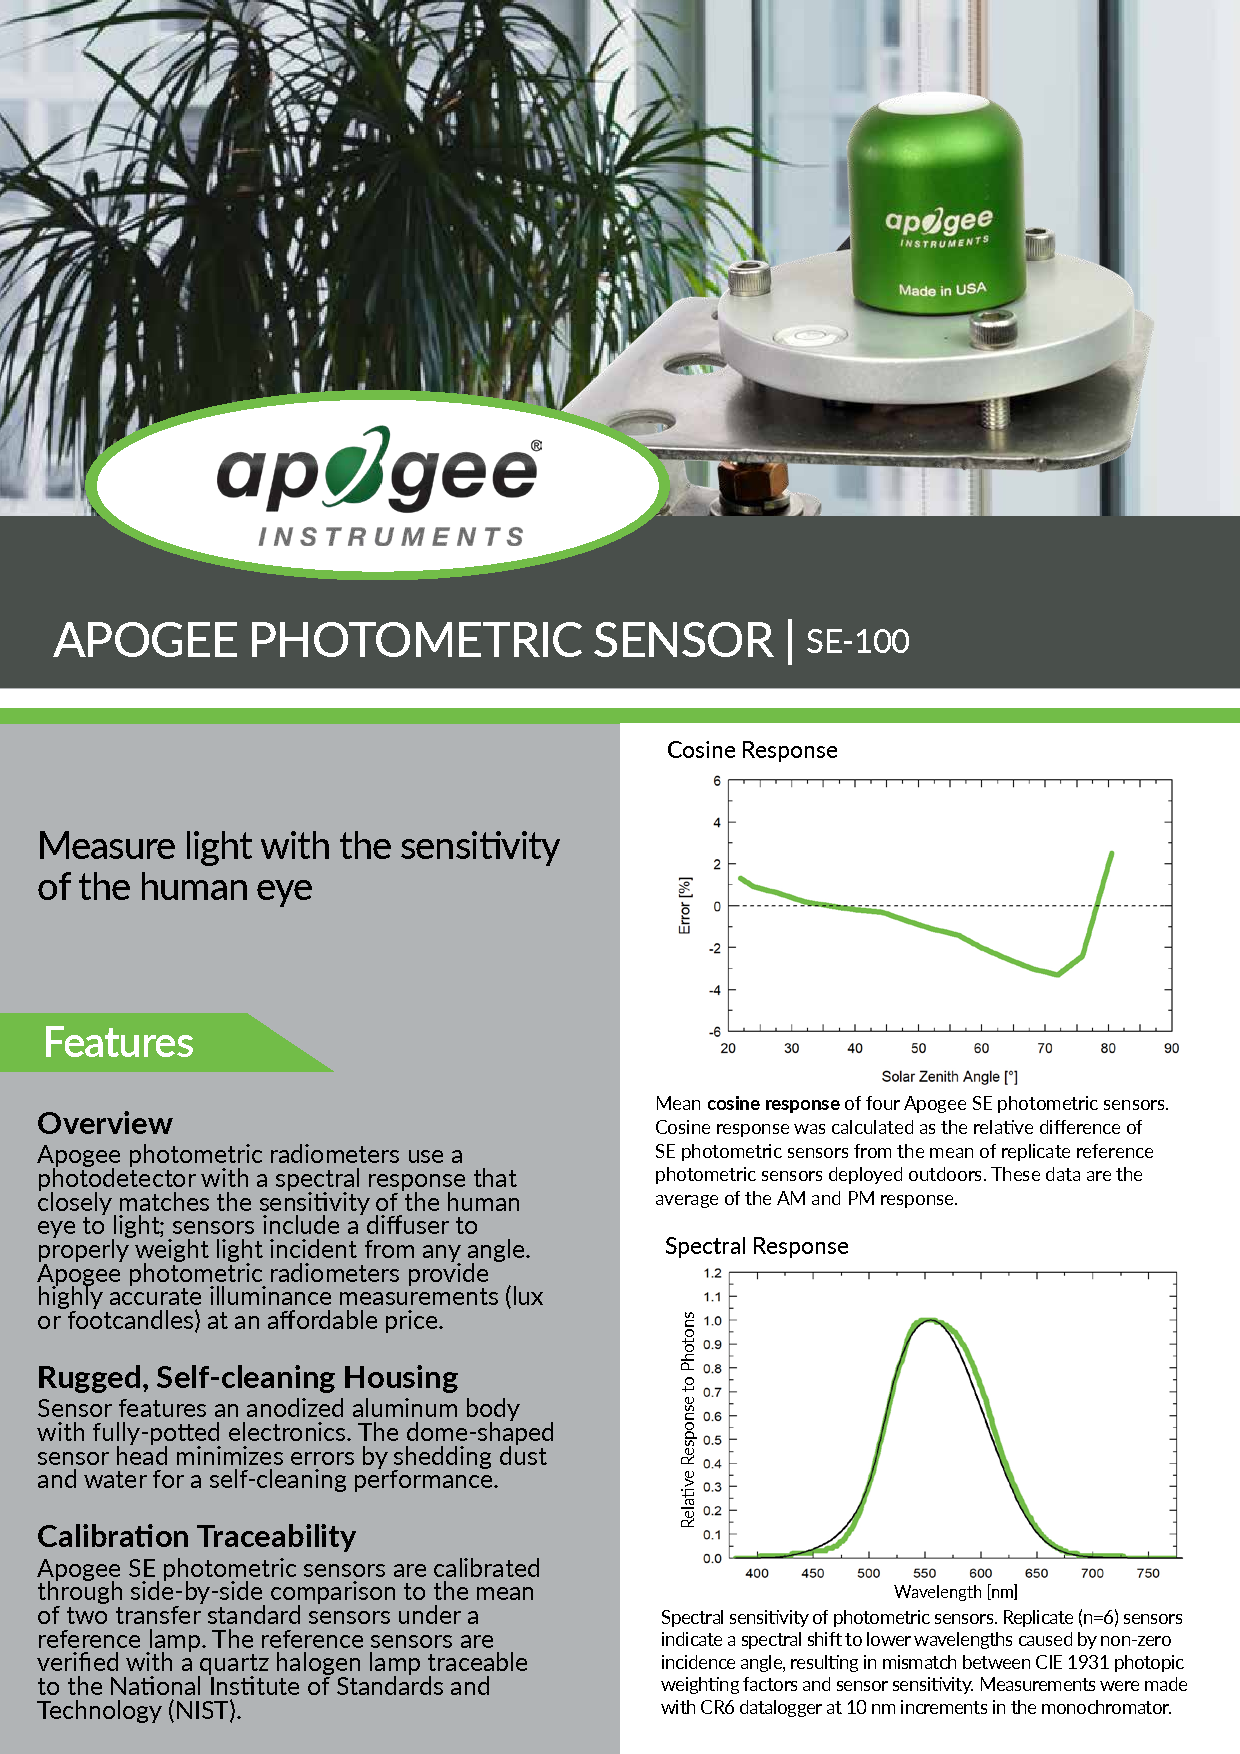
\includegraphics[width=0.8\textwidth]{Appendices/Apogee_SE-100-SS_spec-sheet_p1.pdf}
\caption*{Apogee specifications sheet for SE-100-SS, p.1.}
\end{figure}


\newpage
\begin{figure}[!h]
\centering
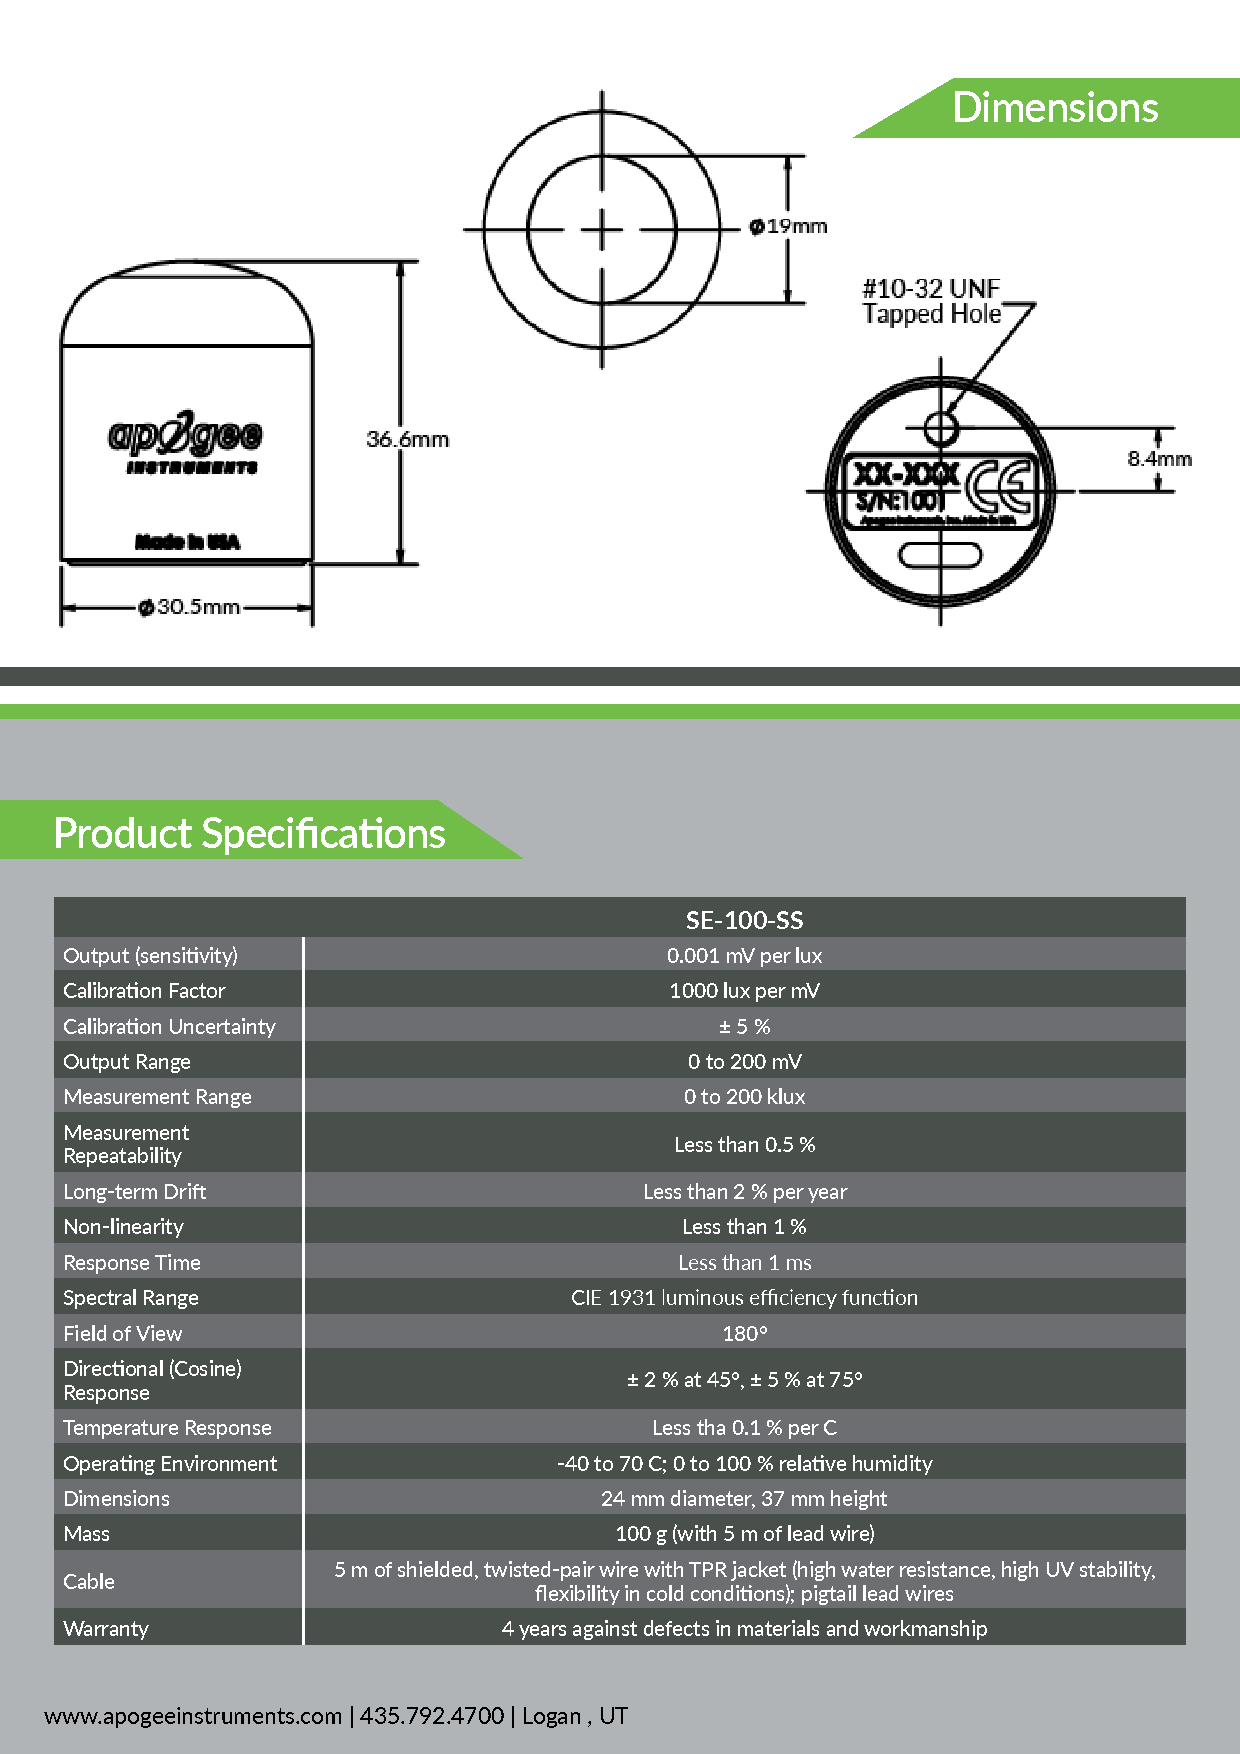
\includegraphics[width=0.8\textwidth]{Appendices/Apogee_SE-100-SS_spec-sheet_p2.pdf}
\caption*{Apogee specifications sheet for SE-100-SS, p.2.}
\end{figure}



%%%%%%%%%%%%%% CODE PAINT %%%%%%%%%%%%%%

\newpage
\section[\hspace{0.3cm}Description of the code paint]{ Appendix: Description of the code given to each paint mixture}
\label{app:ch4_code-paint}

\begin{figure}[!h]
\centering
\includegraphics[width=0.6\textwidth]{Appendices/Figures/paint_code_explanation.png}
\caption*{Explanation of the paint code.}
\end{figure}



%%%%%%%%%%%%%% LIGHT BOX - DARK SAMPLES %%%%%%%%%%%%%%

\newpage
\section[\hspace{0.3cm}Light box experiments - Samples kept in the dark]{ Appendix: Light box experiments - Samples kept in the dark}
\label{app:ch4_LB_dark_samples}

\begin{table}[!h]
\centering
\caption*{Paint-out samples used in the light box experiments: dark samples.}
\begin{tabular}{C{1cm}C{2.2cm}C{1.7cm}C{2cm}C{1.7cm}C{1cm}C{1.7cm}}
\toprule[0.4mm]
\textbf{Code paint$^a$} & \textbf{Paint tubes (p1-p2)} & \textbf{Ratio (p1-p2)} & \textbf{Binding medium} & \textbf{Thickness (\unit{\um})$^b$} & \textbf{Box} & \textbf{Sample Id} \\ \midrule
\multirow{2}{1cm}{\centering P100} & \multirow{2}{2.2cm}{\centering \gls{CYL2b}} & \multirow{2}{1.7cm}{\centering 1-0} & \multirow{2}{2cm}{\centering Linseed oil} & \multirow{2}{1.7cm}{\centering 100} & Box 1 & PO006 \\ 
& & & & & Box 2 & PO066 \\\hline
P140.5 & \multirow{5}{2.2cm}{\centering \gls{CYL2b}-\acrshort{ZW2}} & 0.05-0.95 & \multirow{5}{2cm}{\centering Poppyseed oil} & \multirow{5}{1.7cm}{\centering 100} & Box 2 & PO071 \\
P141 & & 0.1-0.9 & & & Box 1 & PO007 \\ 
P142 & & 0.2-0.8 & & & Box 1 & PO011 \\
P145 & & 0.5-0.5 & & & Box 1 & PO014 \\
P149 & & 0.9-0.1 & & & Box 1 & PO017 \\\hline
P130.5 & \multirow{4}{2.2cm}{\centering \gls{CYL2b}-\acrshort{ZW1}} & 0.05-0.95 & \multirow{4}{2cm}{\centering Linseed oil} & \multirow{4}{1.7cm}{\centering 100} & Box 2 & PO071 \\
P131 & & 0.1-0.9 & & & Box 1 & PO029 \\ 
\multirow{2}{1cm}{\centering P135} & & \multirow{2}{2cm}{\centering 0.5-0.5} & & & Box 1 & PO030 \\
& & & & & Box 2 & PO062 \\\hline
P151 & \multirow{2}{2.2cm}{\centering \gls{CYL2b}-\acrshort{LW}} & 0.1-0.9 & \multirow{2}{2cm}{\centering Linseed oil} &  \multirow{2}{1.7cm}{\centering 100} & \multirow{2}{1cm}{\centering Box 1} & PO023 \\  
P155 & & 0.5-0.5 & & & & PO025 \\\hline
P199 & \multirow{2}{2.2cm}{\centering \gls{CYL2b}-\acrshort{BB}} & 0.9-0.1 & \multirow{2}{2cm}{\centering Linseed oil} & \multirow{2}{1.7cm}{\centering 100} & \multirow{2}{1cm}{\centering Box 1} & PO046 \\
P199.9 & & 0.99-0.01 & & & & PO048 \\\hline
\multirow{4}{1cm}{\centering P200} & \multirow{4}{2.2cm}{\centering \gls{CYSig}} & \multirow{4}{1.7cm}{\centering 1-0} & \multirow{4}{2cm}{\centering Linseed oil} & 100 & Box 1 & PO020 \\
& & & & 50 & \multirow{3}{1cm}{\centering Box2} & PO115 \\
& & & & 100 & & PO065 \\
& & & & 200 & & PO118 \\\hline
P125 & \multirow{2}{2.2cm}{\centering \gls{CYL2b}-\gls{CYSig}} & 0.5-0.5 & \multirow{2}{2cm}{\centering Linseed oil} & \multirow{2}{1.7cm}{\centering 100} & \multirow{2}{1cm}{\centering Box 1} & PO033 \\
P121 & & 0.1-0.9 & & & & PO038 \\\hline
P235 & \gls{CYL2b}-\acrshort{ZW1} & 0.5-0.5 & Linseed oil & 100 & Box 1 & PO039 \\\hline
P255 & \gls{CYL2b}-\acrshort{LW} & 0.5-0.5 & Linseed oil & 100 & Box 1 & PO042 \\\hline
P300 & \acrshort{ZW1} & \multirow{3}{1.7cm}{\centering 1-0} & Linseed oil & \multirow{3}{1.7cm}{\centering 100} & \multirow{3}{1cm}{\centering Box2} & PO052 \\
P400 & \acrshort{ZW2} & & Poppyseed oil & & & PO055 \\
P500 & \acrshort{LW} & & Linseed oil & & & PO057 \\\hline
P700 & \acrshort{Eo1} & \multirow{3}{1.7cm}{\centering 1-0} & \multirow{3}{2cm}{\centering Linseed oil} & 100 & \multirow{3}{1cm}{\centering Box2} & PO093 \\
\multirow{2}{1cm}{\centering P800} & \multirow{2}{2.2cm}{\centering \acrshort{Rev-Eo-1A}} & & & 100 & & PO097 \\
& & & & 200 & & PO123 \\
\bottomrule[0.4mm]
\end{tabular}
\footnotesize{\\ \textsuperscript{a} An explanation of the codes is given in Appendix \ref{app:ch4_code-paint}. \\ \textsuperscript{b} Thickness when the paint is wet. The paint film tends to shrink during the drying process.}
\label{tab:LB_info_PO-dark}
\end{table}


%%%%%%%%%%%%%% PHOTOS CROSS-SECTIONS PO %%%%%%%%%%%%%%


\newpage
\section[\hspace{0.3cm}Photographs of cross-section samples]{ Appendix: Photographs of cross-section samples}
\label{app:ch4_PO_thickness}

\begin{figure}[!h]
\centering
\includegraphics[width=\textwidth]{Appendices/Figures/2021-05-03_CS.001_PO.003_x6.6_aged.jpg}
\caption*{Photograph of cross-section CS.001 - sample PO003 - \gls{CYL2b}, made with a drawdown metallic bar set to a thickness of 100\unit{\um}.}
\label{fig:CS.001_PO003}
\end{figure}



%%%%%%%%%%%%%% CY PIGMENTS FABRICATION %%%%%%%%%%%%%%

\newpage
\section[\hspace{0.3cm}Report on the fabrication of chrome yellow (\acrshort{CYL2b}) pigment]{ Appendix: Report on the fabrication of chrome yellow (\gls{CYL2b}) pigment}
\label{app:ch4_making_CYL2b_pigments}

\begin{figure}[!h]
\centering
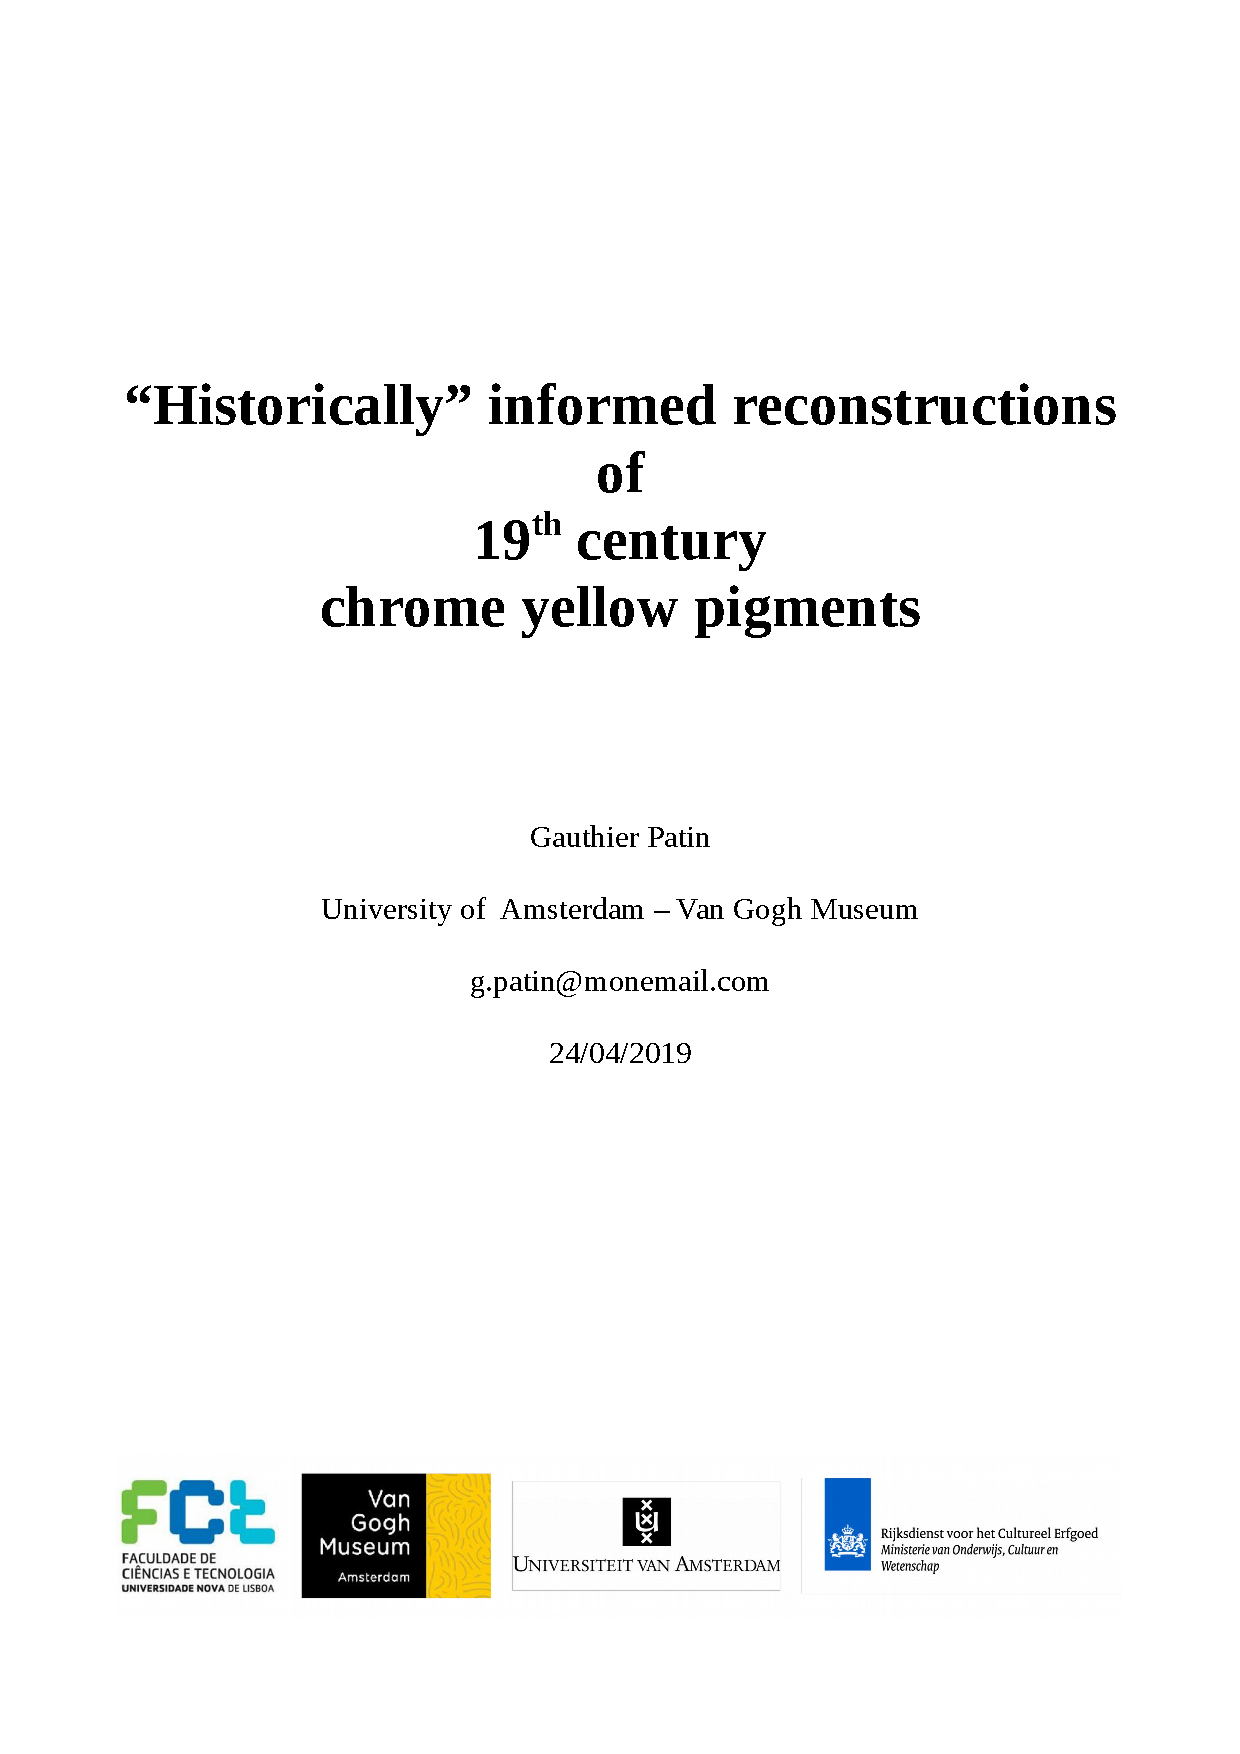
\includegraphics[width=0.8\textwidth]{Appendices/2019-04-24_CY_Pigment_Fabrication_Report_p1.pdf}
%\caption[\hspace{0.3cm}]{Apogee specifications sheet for SP-110-SS, p.2.}
%\label{fig:sMFT_3Dprints_1-4_photos}
\end{figure}

\includepdf[pages=2-3]{Appendices/2019-04-24_CY_Pigment_Fabrication_Report.pdf}



%%%%%%%%%%%%%% CY PAINTS FABRICATION %%%%%%%%%%%%%%

\newpage
\section[\hspace{0.3cm}Report on the fabrication of chrome yellow (\acrshort{CYL2b}) paint]{ Appendix: Report on the fabrication of chrome yellow (\gls{CYL2b}) paint}
\label{app:ch4_making_CYL2b_paints}


\begin{figure}[!h]
\centering
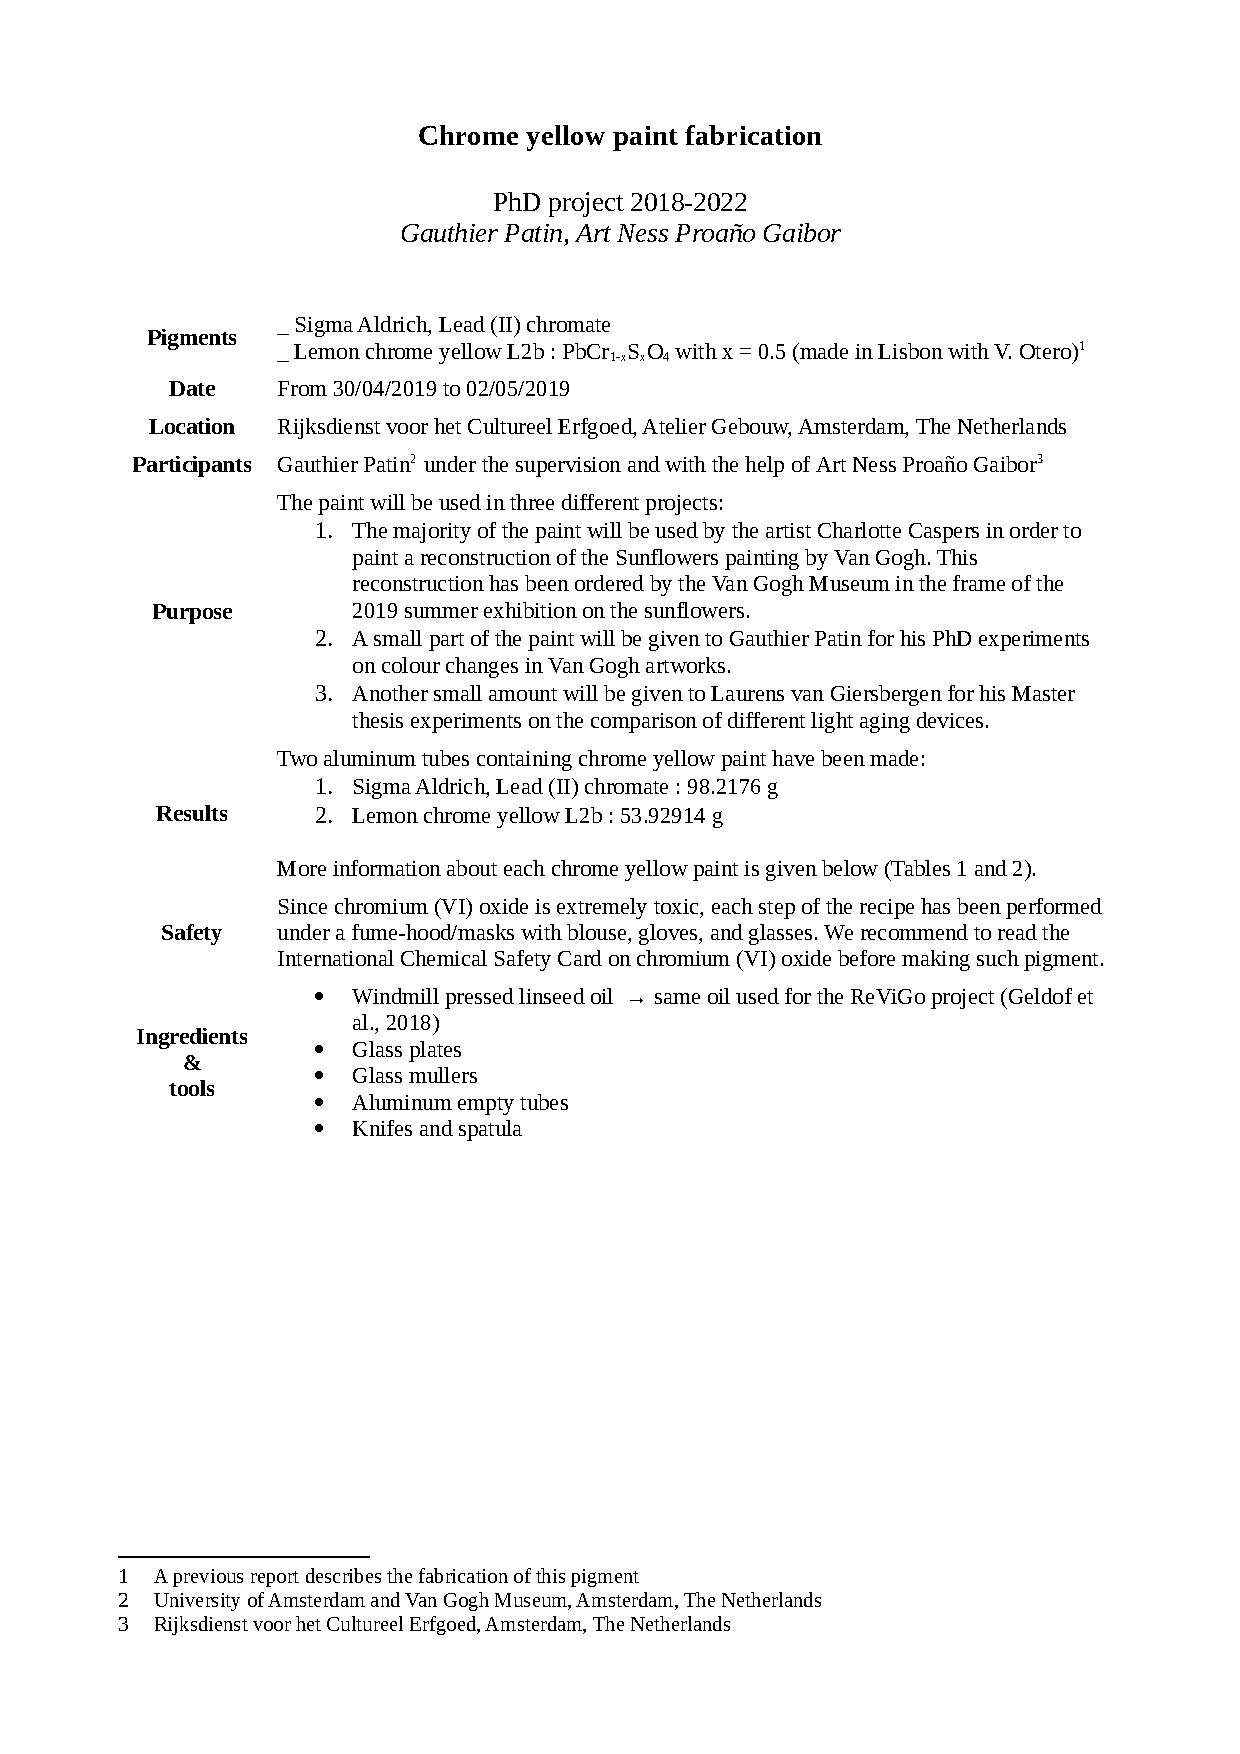
\includegraphics[width=0.85\textwidth]{Appendices/2019-05-16_CY_Paint_Making_Report_p1.pdf}
%\caption[\hspace{0.3cm}]{Apogee specifications sheet for SP-110-SS, p.2.}
%\label{fig:sMFT_3Dprints_1-4_photos}
\end{figure}

\includepdf[pages=2-3]{Appendices/2019-05-16_CY_Paint_Making_Report.pdf}



%%%%%%%%%%%%%% EOSIN PAINT FABRICATION %%%%%%%%%%%%%%

\newpage
\section[\hspace{0.3cm}Report on the fabrication of the eosin paint]{ Appendix: Report on the fabrication of the eosin paint}
\label{app:ch4_making_eosin}

As mentioned in the dissertation, the eosin pigment has been created by Alba Alvarez-Martin and Teresa Scovacricchi at the \gls{UA} according to a recipe found in \citet{claro_identification_2010}.\\

Ingredients:
\begin{itemize}
\item Sodium hydroxide (NaOH)
\item Eosin Y (bought from Sigma)
\item Aluminum chloride hexahydrate
\end{itemize}

\vspace{1cm}

Process steps:
\begin{enumerate}
\item Dissolve the eosin Y pigments in basic water (Figure (a))
\item Add the aluminum in the solution (Figure (b))
\item Set it aside, and let the sedimentation process happens for a few hours (Figure (c) \& (d))
\item Filter the solution and let the pigment to dry
\item Grind the pigment
\end{enumerate}

\vspace{1.5cm}

\begin{figure}[!h]
  \centering
  
  \subfigure(a){\includegraphics[width=0.2\textwidth]{Appendices/Figures/Scovacricchi_2020_eosin-making_eosin-dissolution.png}} 
  \subfigure(b){\includegraphics[width=0.2\textwidth]{Appendices/Figures/Scovacricchi_2020_eosin-making_adding-AL-salt.png}} 
  \subfigure(c){\includegraphics[width=0.2\textwidth]{Appendices/Figures/Scovacricchi_2020_eosin-making_sedimentation.png}}
  \subfigure(d){\includegraphics[width=0.2\textwidth]{Appendices/Figures/Scovacricchi_2020_eosin-making_sedimented.png}}

  \caption*{(a) Dissolve the eosin Y in basic water (b) Add the aluminum salt (c) Sedimentation phase (d) After sedimentation (Photographic credits Teresa Scovacricchi).}
 
\end{figure}


\vspace{1.5cm}

After receiving the eosin pigment, I created the eosin paint as described below:
\begin{enumerate}
\item Pour the eosin pigment on a glass plate and add a few drop of linseed oil, which was made during the \gls{REVIGO} project \citep{geldof_reconstructing_2018}. 
\item Mix the oil and the pigment with a spatula (Figure below - e)
\item Then grind the pigment with a glass muller (Figure below - f)
\end{enumerate} 


\begin{figure}[!h]
  \centering
  
  \subfigure(e){\includegraphics[width=0.45\textwidth]{Appendices/Figures/2022-04-11_02_eosinA+oil.JPG}} 
  \subfigure(f){\includegraphics[width=0.45\textwidth]{Appendices/Figures/2022-04-11_04_Eo1.JPG}} 

  \caption*{(e) Mix the eosin with linseed oil (f) Grinding phase.}
\label{fig:eosin_making_paint}
\end{figure}

%%%%%%%%%%%%%% METHODOLOGY PHOTOGRAPHS %%%%%%%%%%%%%%

\newpage
\section[\hspace{0.3cm}Methodology of the photographs]{ Appendix: Methodology of the photographs}
\label{app:ch4_methodology_photos}

\begin{table}[!h]
\centering 
\caption*{Parameters of the camera and photos.}
\begin{tabular}{R{6cm}L{6cm}}
\toprule[0.4mm]
\textbf{Camera brand} & Canon \\
\textbf{Camera model} & EOS 5D Mark III \\
\textbf{Objective} & Canon EF 50mm f/1.4 USM \\
\textbf{Exposure Time} & 1/125 s \\
\textbf{F-number} & F13 \\
\textbf{ISO} & 100 \\
\textbf{Colour checker} & X-rite SG card \\
\textbf{File type} & TIFF (16 bits) \\
\bottomrule[0.4mm]
\end{tabular}
\label{tab:photos_params}
\end{table}

Steps - Capture:
\begin{enumerate}
\item Take a photo of the colour checker
\item Take an empty photo of the table (flatfielding)
\item Take a photograph of each object
\end{enumerate}

\vspace{1cm}

Steps - Processing:
\begin{enumerate}
\item White balance (done with Canon software)
\item Flatfielding (done with NIP2 software)
\item Create an ICC profile using the photo of the flatfielded colour checker. In a terminal, perform the following two commands.
\begin{enumerate}
\item scanin method (see Figure below)
\item colprof method (see Figure below)
\end{enumerate}
\item Apply the ICC profile to the other photos (output profile: eci\_RGBv2)
\end{enumerate}

\begin{figure}[!h]
\centering
\includegraphics[width=\textwidth]{Appendices/Figures/Scanin_method_terminal.png}
\caption*{Scaning method.}
\end{figure}


\begin{figure}[!h]
\centering
\includegraphics[width=\textwidth]{Appendices/Figures/Colprof_method_terminal.png}
\caption*{Colprof method.}
\end{figure}

%%%%%%%%%%%%%% APOGEE SP-110-SS %%%%%%%%%%%%%%

\newpage
\section[\hspace{0.3cm}Information about the Apogee SP-110-SS sensor]{ Appendix: Information about the Apogee SP-110-SS sensor}
\label{app:ch4_apogee_SP-110-SS}

\begin{figure}[!h]
\centering
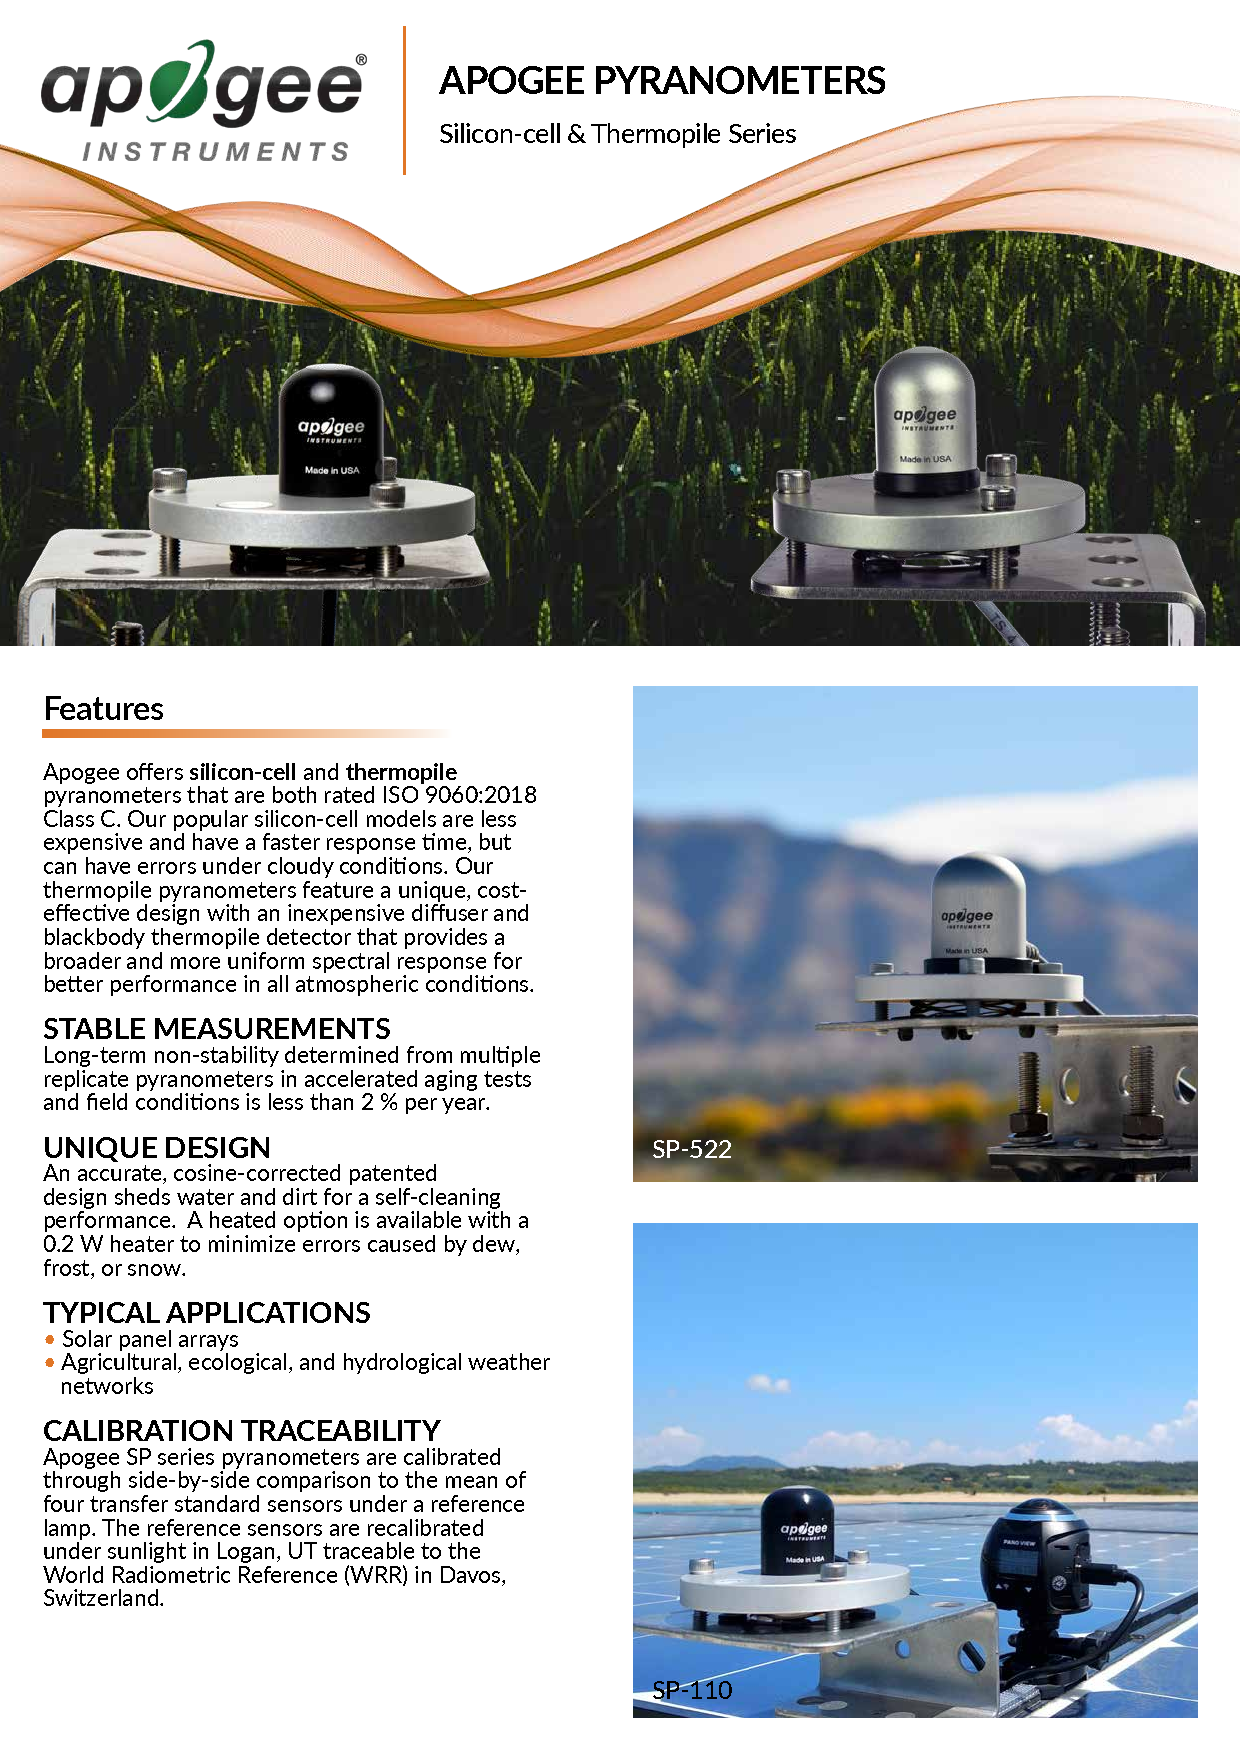
\includegraphics[width=0.8\textwidth]{Appendices/Apogee_SP-110-SS_spec-sheet_p1.pdf}
\caption*{Apogee specifications sheet for SP-110-SS, p.1.}
\end{figure}

\newpage

\begin{figure}[!h]
\centering
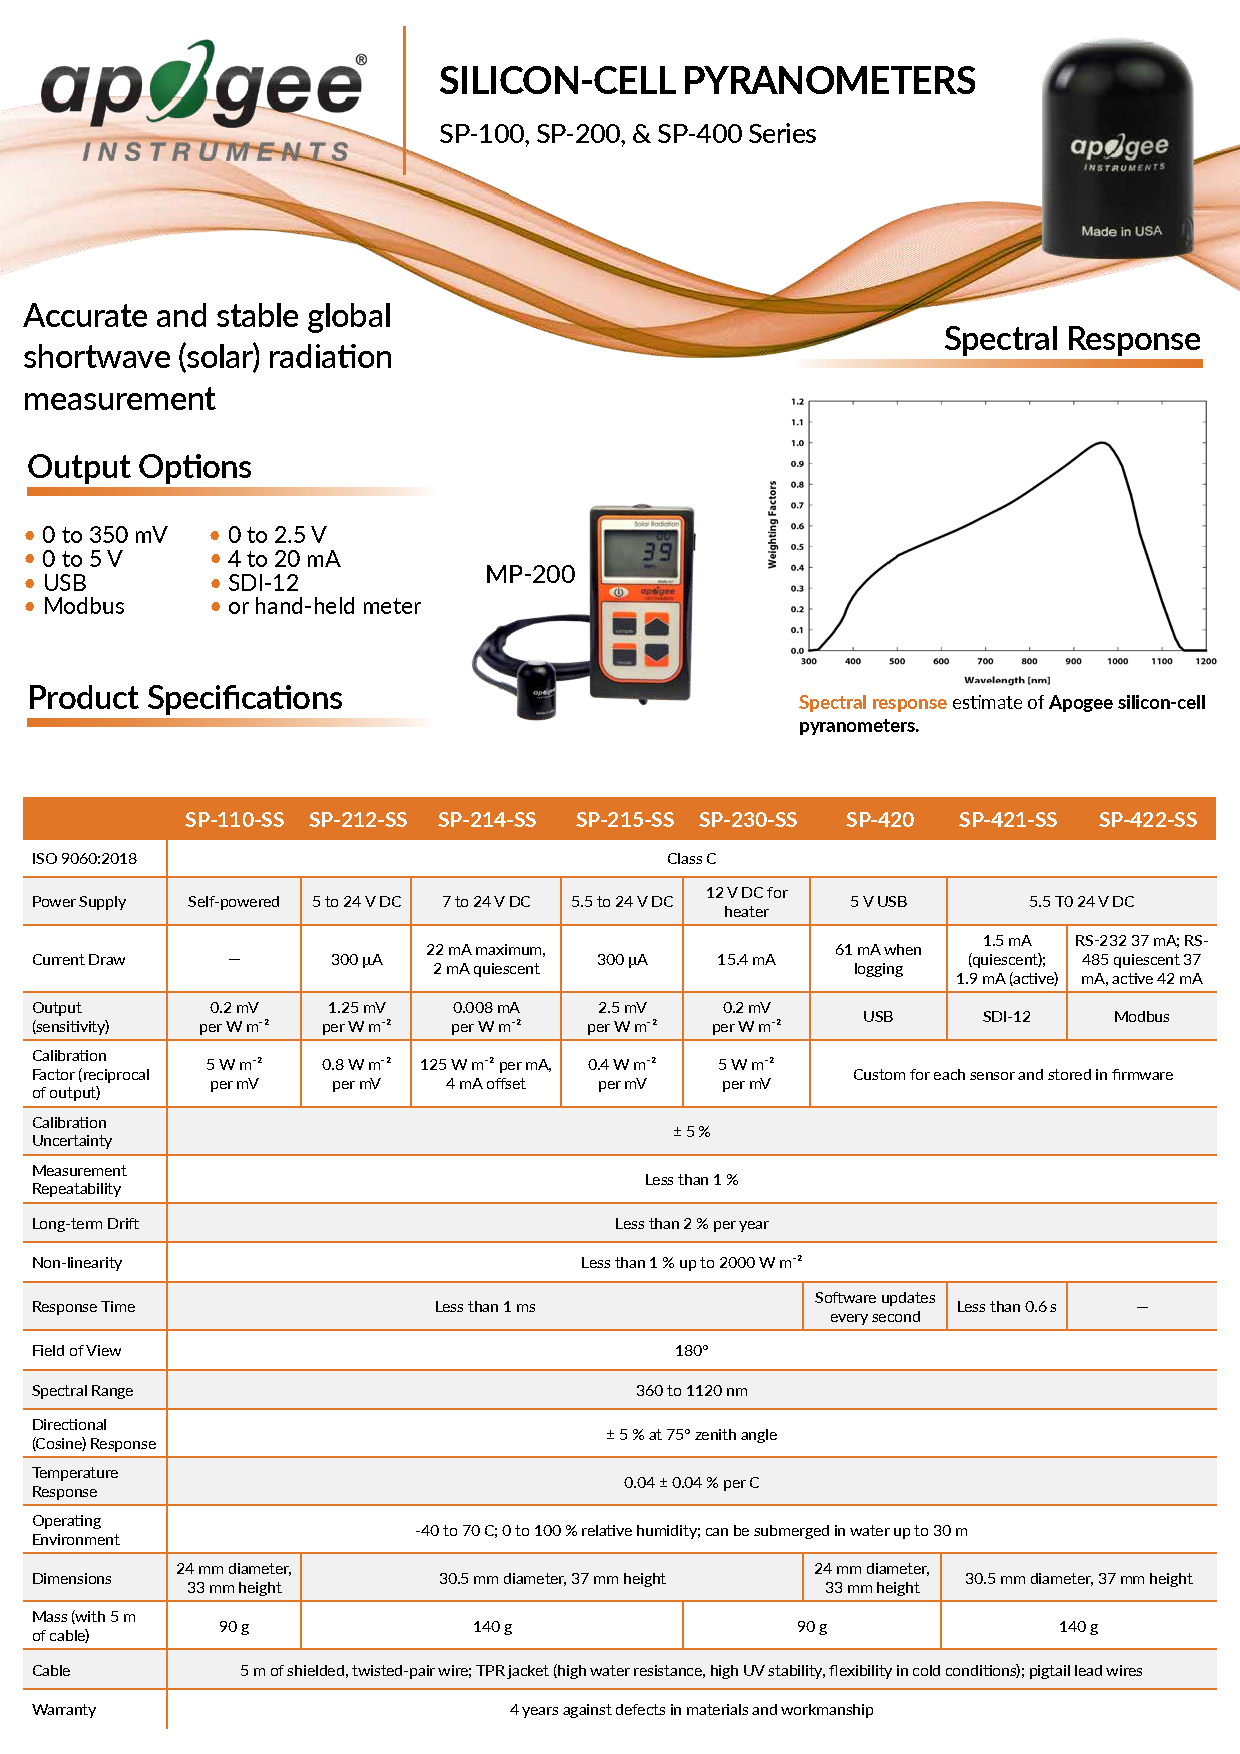
\includegraphics[width=0.8\textwidth]{Appendices/Apogee_SP-110-SS_spec-sheet_p2.pdf}
\caption*{Apogee specifications sheet for SP-110-SS, p.2.}
\end{figure}



%%%%%%%%%%%%%% dR_VIS CURVES %%%%%%%%%%%%%%

\newpage
\section[\hspace{0.3cm}Comparison of the \dRvis curves for each sample]{ Appendix: Comparison of the \dRvis curves for each sample.}
\label{app:ch4_LB-DL-MF_all_dRvis}

\begin{figure}[!h]
\centering
\includegraphics[width=\textwidth]{Appendices/Figures/Comparison_DL-LB-MF_all_aged_dR_VIS.png}
\caption*{\dRvis for each sample used in the light box, daylight, and MFT experiments. Equivalent to Figure \ref{fig:DL-LB-MF_all_aged_dE00} but with \dRvis values instead of \dEOO.}
\label{fig:DL-LB-MF_all_aged_dRvis}
\end{figure}



%%%%%%%%%%%%%% DAYLIGHT EXP - BWS %%%%%%%%%%%%%%

\newpage
\section[\hspace{0.3cm}Results of the daylight experiments for the \gls{BWS}]{ Appendix: Results of the daylight experiments for the \gls{BWS}.}
\label{app:ch4_DL_BW1_dEOO}

\begin{figure}[!h]
\centering
\includegraphics[width=\textwidth]{Appendices/Figures/DL_BWS_aged_dE00.png}
\caption*{Daylight experiments - \gls{BWS} samples.}
\label{fig:DL_BWS_aged_dE00}
\end{figure}

\end{appendices}